%% IEEE Journal of Biomedical and Health Informatics -- regular paper (single-blind).
%% Build: pdflatex main && bibtex main && pdflatex main && pdflatex main
%% Content source: the earlier manuscript (every number verified against results/final/*.txt|*.md);
%% this file re-typesets and re-frames that manuscript without changing any number or claim.
\documentclass[journal]{IEEEtran}

\usepackage[T1]{fontenc}
\usepackage{cite}
\usepackage{amsmath,amssymb}
\usepackage{booktabs}
\usepackage{array}
\usepackage{graphicx}
\usepackage{tikz}
\usetikzlibrary{positioning,arrows.meta,calc}
\usepackage{url}
\usepackage{placeins}
\usepackage{needspace}
\usepackage[hidelinks]{hyperref}
\hypersetup{pdfauthor={Sharoon Sharif},pdftitle={One Checkpoint for Complete, Slide-Only and RNA-Only Patients: Auditing and Training Histology\textendash Transcriptomics Survival Models for Missing Inputs}}

\newcommand{\pq}{PathQ-Former}
\newcommand{\cindex}{C-index}
\newcommand{\pmv}[2]{#1\,$\pm$\,#2}
\newcolumntype{R}[1]{>{\raggedright\arraybackslash}p{#1}}

\begin{document}

\title{One Checkpoint for Complete, Slide-Only and RNA-Only Patients: Auditing and Training Histology--Transcriptomics Survival Models for Missing Inputs}

\author{Sharoon~Sharif%
\thanks{Manuscript received October XX, 2026.}%
\thanks{S. Sharif is with the Department of Electrical Engineering and Computer Science, Alabama A\&M University, Normal, AL 35762 USA, and with Faith Comes By Hearing, Albuquerque, NM USA (e-mail: ADD-EMAIL).}}

\markboth{Submitted to the IEEE Journal of Biomedical and Health Informatics}%
{Sharif: One Checkpoint for Complete, Slide-Only and RNA-Only Patients}

\maketitle
\bstctlcite{IEEEexample:BSTcontrol}

\begin{abstract}
Survival models that fuse whole-slide images with transcriptomics are evaluated on patients who have both inputs, whereas a hospital cohort also holds slide-only and RNA-only patients. Two questions are then open: does the fused model use both inputs, and what happens when one is missing? We audit this on five cohorts of The Cancer Genome Atlas under one equal-budget, three-seed protocol by re-evaluating trained checkpoints with an input removed or permuted across patients. Under this protocol, the official SurvPath implementation ranks patients the same way when its RNA input is permuted (\cindex{} change $+0.001$) but loses 0.068 when the slide is permuted and falls to 0.47--0.52 without it. A query-bottleneck fusion model trained with learned null codes and modality dropout is equally invariant to RNA removal but loses only 0.030 without the slide. Adding auxiliary unimodal heads makes the fused prediction respond to RNA ($-0.023$ under permutation); the resulting single trained model (one checkpoint) keeps a \cindex{} of 0.54--0.62 with either input removed and moves at most 0.025 when half the patients lack a modality, so one model serves complete, slide-only and RNA-only patients. With both inputs it does not detectably beat an RNA-only multilayer perceptron or a late-fusion ensemble, and its $+0.036$ margin over the untuned SurvPath is significant under the Wilcoxon test but not the $t$-test. Replayed on stored training histories, validation-loss early stopping would have cost the two variants 0.06--0.09 \cindex{} and SurvPath nothing. Code, per-run results and checkpoints are released.
\end{abstract}

\begin{IEEEkeywords}
Computational pathology, missing modality, model auditing, multimodal fusion, survival analysis, transcriptomics, whole-slide images.
\end{IEEEkeywords}

\section{Introduction}
\label{sec:intro}

\IEEEPARstart{I}{n} routine care, tumour sequencing is ordered for a subset of patients and slide digitisation is incomplete, so a prognostic cohort is rarely complete: some patients have a whole-slide image (WSI), some have bulk RNA-seq and some have both. Prognostic models that fuse the phenotype recorded by histology with the molecular state recorded by transcriptomics report higher concordance than either modality alone on most cohorts of The Cancer Genome Atlas (TCGA)~\cite{chen2022pancancer,jaume2024survpath,song2024mmp}: pathology foundation models~\cite{chen2024uni,xu2024gigapath,vorontsov2024virchow} turn a gigapixel WSI into a few thousand frozen patch embeddings, and co-attention between patch tokens and gene or pathway tokens~\cite{chen2021mcat,jaume2024survpath} relates the two sets. Such models are evaluated on patients who have both inputs, which leaves two questions open that an accuracy table cannot answer. Does the fused model use both inputs? A concordance index (\cindex{}) measures how well predicted risks rank patients; it cannot show which input produced the ranking, so a model that silently ignores one input is a hidden failure. And what happens when one input is missing? A model that needs both inputs cannot serve the incomplete patients.

We answer both questions with an input-use audit: every trained checkpoint is re-evaluated with one input removed, with one input permuted across patients, and with a random fraction of patients lacking a modality, and its fused risk scores are correlated with the risks of its own single-input evaluations. Applied under one protocol to the official SurvPath implementation~\cite{jaume2024survpath}, the audit finds that SurvPath's ranking does not respond to its RNA input ($\Delta$\cindex{} $+0.001$ under permutation across patients) and collapses when the slide is permuted ($\Delta$\cindex{} $-0.068$) or removed (\cindex{} 0.47--0.52).

The practical result is a training recipe that lets one trained model serve complete, slide-only and RNA-only patients. We train one query-bottleneck fusion model, \pq{}, in two variants that differ only in training. With learned null codes and modality dropout alone, the model is as invariant to RNA as SurvPath ($\Delta$\cindex{} $0.000$ with RNA removed) but no longer collapses without the slide ($-0.030$ instead of SurvPath's $-0.073$). Adding auxiliary unimodal survival heads makes the fused prediction respond to RNA ($-0.023$ under permutation); the resulting checkpoint keeps a \cindex{} of 0.54--0.62 with either input removed and changes by at most 0.025 when half of the patients lack a modality. With both inputs present, neither variant is detectably better than an RNA-only multilayer perceptron (MLP) or a late-fusion ensemble of two unimodal models, so the recipe buys coverage of incomplete patients, not accuracy. Our contributions are:
\begin{itemize}
\item A one-checkpoint training recipe assembled from existing components (null codes, modality dropout, auxiliary unimodal heads), with matched-variant evidence on where its missing-modality robustness comes from (Sections~\ref{sec:missing} and~\ref{sec:where}).
\item An input-use audit (removal, permutation across patients, risk-score correlation; 3 seeds $\times$ 5 folds $\times$ 5 cohorts) applied to a published co-attention model under an equal-budget protocol (Section~\ref{sec:audit}). SurvPath's ranking, as trained under this protocol, does not respond to its RNA input; a high fused \cindex{} does not show that both modalities are used.
\item Protocol evidence that this literature rarely reports (Sections~\ref{sec:accuracy} and~\ref{sec:selection}): equal-budget accuracy with seed-aware statistics (seed-averaged 25-fold paired tests with bootstrap confidence intervals and Holm correction), and a post-hoc replay of checkpoint selection on event-poor folds from the stored training histories.
\end{itemize}

\textit{Scope of claims.} SurvPath was run with its published hyper-parameters and was not re-tuned under our protocol. \pq{}'s hyper-parameters were developed on the bladder cohort (BLCA) under a 10-epoch budget, and the auxiliary-head variant and its loss weight were adopted after the 20-epoch results on all five cohorts had been seen, so both variants are reported as co-primary and no accuracy superiority over SurvPath is claimed. The training recipe has not been applied to SurvPath. All results are on TCGA with frozen UNI2-h features, simulated missingness is random and therefore uninformative, and no clinical covariates are modelled.

\section{Related Work}
\label{sec:related}

\textit{Fusion of WSIs and genomics.} WSIs are processed as bags of patches under multiple-instance learning: attention-based MIL (ABMIL)~\cite{ilse2018abmil}, CLAM~\cite{lu2021clam} and TransMIL~\cite{shao2021transmil} pool patch features from self-supervised~\cite{wang2022ctranspath} or foundation-model encoders trained on $10^8$ patches or more~\cite{chen2024uni,xu2024gigapath,vorontsov2024virchow}. Early fusion work concatenated convolutional neural network (CNN) and genomic features~\cite{mobadersany2018predicting} or combined unimodal representations with Kronecker products and gating~\cite{chen2022pathomic}; a pan-cancer study found that fusion improved concordance in 12 of 14 cancer types~\cite{chen2022pancancer}. MCAT~\cite{chen2021mcat} introduced co-attention from functional gene groups to patches; SurvPath~\cite{jaume2024survpath} replaced the groups with Reactome and Hallmark pathway tokens and modelled dense pathway--patch interactions in one Transformer; MOTCat~\cite{xu2023motcat}, CMTA~\cite{zhou2023cmta}, PIBD~\cite{zhang2024pibd} and MMP~\cite{song2024mmp}, which reports gains over SurvPath, vary the interaction, and continually evolved multimodal foundation models extend the setting~\cite{peng2025continual}. Two-bank learned-query fusion over patches and pathways already exists in APL~\cite{liu2025apl}; the query bottleneck used here is not claimed as new.

\textit{Missing modalities in multimodal survival.} Modality dropout was introduced for gesture recognition~\cite{neverova2016moddrop} and applied to pan-cancer prognosis by Cheerla and Gevaert~\cite{cheerla2019deep} and MultiSurv~\cite{valesilva2021long}. Ma et al.~\cite{ma2022robust} showed that multimodal Transformers are not robust to missing inputs by default; SMIL~\cite{ma2021smil}, ShaSpec~\cite{wang2023shaspec} and missing-aware prompts~\cite{lee2023prompt} address it with meta-learning, shared--specific features or prompt tokens. For WSIs and genomics, G-HANet~\cite{wang2024ghanet} distils genomic knowledge into a histology-only model, and recent work binds incomplete modalities~\cite{qu2024binding}, distils prompts~\cite{xu2025dispro}, learns conditional latent variables~\cite{zhou2025ldcvae}, uses prototype-guided cross-modal knowledge~\cite{liu2025prosurv}, memory-augmented hypergraphs~\cite{qu2025m2surv} or prototype-driven pretraining~\cite{yu2026prime}. None of these audits whether a published co-attention model uses its genomic input, nor tests under equal budgets whether unimodal auxiliary supervision changes that; this is the gap we address.

\textit{Learned queries and modality imbalance.} A set of learned vectors that cross-attend to a large input and return a fixed-size summary appears as inducing points~\cite{lee2019set}, object queries~\cite{carion2020detr}, the Perceiver latent array~\cite{jaegle2021perceiver}, the Perceiver Resampler~\cite{alayrac2022flamingo}, the Q-Former~\cite{li2023blip2} and the prototype banks of APL~\cite{liu2025apl}; the property used here is that the output has a fixed shape, so an absent input can be replaced by a learned tensor of the same shape. Gradient Blending~\cite{wang2020gradientblending} and OGM-GE~\cite{peng2022ogmge} showed that joint training lets one modality dominate and counteract it with per-modality supervision or gradient modulation. The auxiliary unimodal heads used here are unimodal supervision in that tradition, not a new idea; our contribution is to measure what they change in a survival-fusion model under an audit.

\section{Materials and Methods}
\label{sec:setup}

\subsection{Data and Cohorts}
Five TCGA cohorts are used (Table~\ref{tab:cohorts}): bladder urothelial carcinoma (BLCA), breast invasive carcinoma (BRCA), colorectal adenocarcinoma (COADREAD), head and neck squamous cell carcinoma (HNSC) and stomach adenocarcinoma (STAD). Patch embeddings are the released 1,536-d UNI2-h features~\cite{chen2024uni,uni2h,uni2hfeatures}, used as released. The RNA-seq matrices (4,999 genes), clinical metadata and five-fold patient-level splits are those released with SurvPath~\cite{jaume2024survpath}. The primary endpoint is disease-specific survival (DSS) from the TCGA Clinical Data Resource~\cite{liu2018integrated}; overall survival (OS) is secondary. The split is fixed per cohort, so fold $k$ holds the same validation patients for every method and seed, and the number of events in a validation fold ranges from 5 to 45 (median 16).

\begin{table}[!t]
\caption{Cohorts as realised by the DSS splits (every method and seed uses the same five folds). Patients and events per validation fold are the minimum--maximum over the five folds. $^\dagger$Development cohort for \pq{}'s hyper-parameters.}
\label{tab:cohorts}
\centering
\footnotesize
\setlength{\tabcolsep}{2.5pt}
\begin{tabular}{@{}llrrrr@{}}
\toprule
Cohort & Site & Patients & DSS events & Patients/fold & Events/fold \\
\midrule
BLCA$^\dagger$ & bladder & 359 & 113 & 70--75 & 16--25 \\
BRCA & breast & 868 & 60 & 166--182 & 7--20 \\
COADREAD & colorectal & 296 & 37 & 45--71 & 5--13 \\
HNSC & head \& neck & 392 & 117 & 56--126 & 13--45 \\
STAD & stomach & 318 & 84 & 42--101 & 9--33 \\
\bottomrule
\end{tabular}
\end{table}

\subsection{Protocol}
\label{sec:protocol}
One evaluation protocol is applied without change to every method (Supplementary Table~S1). The unit of analysis is the patient, with all slides of a patient concatenated. Every method trains for a fixed budget of 20 epochs and reports the final checkpoint, the convention of MCAT and SurvPath; no checkpoint is selected on the validation fold, which is also the reported fold. The budget was set after inspecting pooled validation curves under a 10-epoch budget (Supplementary Section~S-II), so 10-epoch results are reported as well. Time bins are the quartiles of uncensored training patients, with outer edges $\pm\infty$, reused for validation. The primary metric is Harrell's \cindex{} on continuous time~\cite{harrell1982evaluating,polsterl2020scikit}; the secondary metrics are Uno's inverse-probability-of-censoring-weighted (IPCW) \cindex{}~\cite{uno2011c} truncated at the 75th percentile of training event times, the integrated Brier score~\cite{graf1999assessment} on the interior quartile grid, and the log-rank test at the median risk split (Supplementary Sections~S-III and~S-VI). Three seeds (0, 1, 2) are run, with the fold index added to the seed. Supplementary Section~S-VII lists evaluation pitfalls of survival MIL pipelines that the protocol avoids.

\textit{Statistics.} The three seeds of a fold share its validation patients, so (fold, seed) pairs are not independent replicates~\cite{nadeau2003inference}. The unit of analysis is therefore the (cohort, fold): the \cindex{} of each method is averaged over the seeds available for both methods, the paired difference is formed on each of the 25 folds, and a paired $t$-test, a two-sided exact Wilcoxon signed-rank test and a 95\% percentile-bootstrap confidence interval (CI) of the mean difference (10,000 resamples of folds) are computed over the folds. Per-cohort tests have five folds each; their $p$-values are Holm-adjusted over the five cohorts and are exploratory. ``Mean $\pm$ sd'' in a table is the mean and standard deviation over seeds of the five-fold mean unless the caption says otherwise.

\subsection{Methods}
\label{sec:methods}
Supplementary Table~S2 lists the methods and the seeds run for each. SurvPath (official implementation, 21.2\,M parameters), ABMIL~\cite{ilse2018abmil}, a self-normalizing network (SNN)~\cite{klambauer2017self} on RNA and a two-layer RNA MLP use the hyper-parameters of the SurvPath repository; none was tuned under this protocol. SurvPath samples 4,096 patches per slide, its published setting; \pq{} reads all patches of a patient (6,214 for the median of the 40 profiled BLCA patients, Supplementary Table~S14). SurvPath's \cindex{} values here are those of its official implementation under this protocol and with these patch features, not a reproduction of the values reported by its authors; every comparison in this paper is within the protocol of Section~\ref{sec:protocol}, and the audit describes the checkpoints trained here, not the published model. Two further baselines are a slide-only and an RNA-only \pq{}, trained with the other modality absent, and a late-fusion ensemble that averages the $z$-scored risks of the two (same seed; two seeds). The two co-primary models are \pq{} without auxiliary heads (null codes and modality dropout; 16.9\,M parameters) and \pq{} (the same plus auxiliary heads, $\lambda = 0.5$), trained with AdamW~\cite{loshchilov2019adamw} (SurvPath: RAdam~\cite{liu2020variance}, its published setting; Supplementary Table~S3); each is run with three seeds.

\begin{figure*}[!t]
\centering
% PathQ-Former overview: (a) training, (b) inference.
% Standalone tikzpicture; \input it inside a figure environment.
% Needs tikz with libraries positioning, arrows.meta, calc.
% Colours: histology = blue, transcriptomics = orange, shared parts = neutral gray.
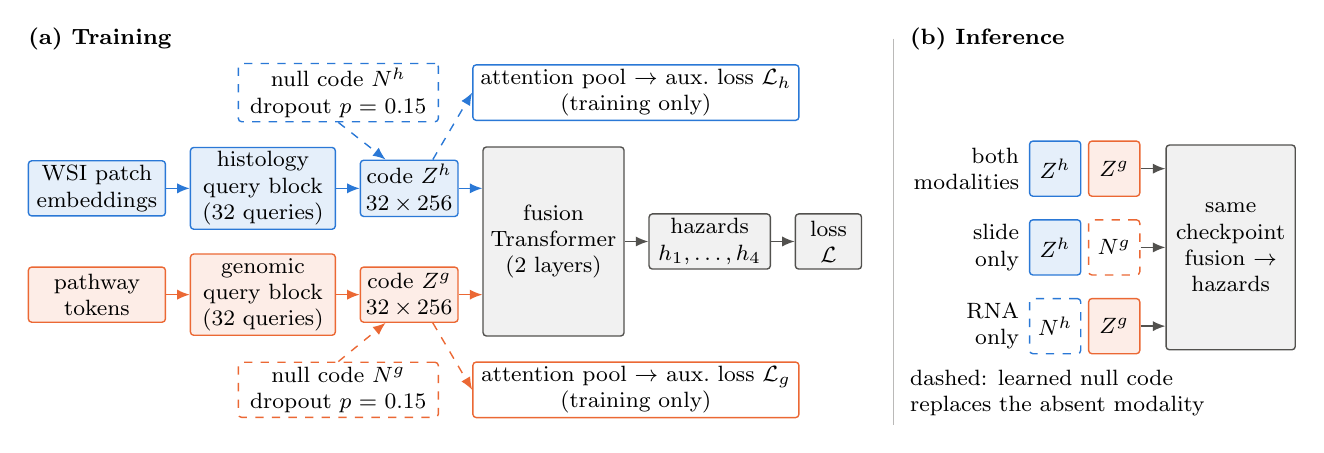
\begin{tikzpicture}[x=1mm, y=1mm, font=\footnotesize, line width=0.5pt,
  >={Latex[length=1.6mm, width=1.3mm]},
  box/.style={draw, rounded corners=1.2pt, align=center, inner xsep=2pt, inner ysep=1.5pt, minimum height=7mm},
  hbox/.style={box, draw=hist, fill=hist!12},
  gbox/.style={box, draw=gen, fill=gen!12},
  nbox/.style={box, draw=neut, fill=neut!8},
  hnull/.style={box, draw=hist, dashed, fill=white},
  gnull/.style={box, draw=gen, dashed, fill=white},
  haux/.style={box, draw=hist, fill=white},
  gaux/.style={box, draw=gen, fill=white},
  chip/.style={box, minimum width=6.5mm, minimum height=5.5mm, inner sep=1pt},
  harr/.style={->, hist},
  garr/.style={->, gen},
  narr/.style={->, neut},
  hdash/.style={->, hist, dashed},
  gdash/.style={->, gen, dashed},
  plab/.style={font=\footnotesize\bfseries, anchor=west, inner sep=0pt},
]
\definecolor{hist}{HTML}{2A78D6}
\definecolor{gen}{HTML}{EB6834}
\definecolor{neut}{HTML}{52514E}

% ---------------- (a) Training ----------------
\node[plab] at (0,32.5) {(a) Training};
\node[hbox, text width=16mm, anchor=west] (wsi) at (0,13.5) {WSI patch\\embeddings};
\node[gbox, text width=16mm, anchor=west] (rna) at (0,0)    {pathway\\tokens};
\node[hbox, text width=17mm, right=3mm of wsi] (qh) {histology\\query block\\(32 queries)};
\node[gbox, text width=17mm, right=3mm of rna] (qg) {genomic\\query block\\(32 queries)};
\node[hbox, text width=11mm, right=3mm of qh] (zh) {code $Z^h$\\$32 \times 256$};
\node[gbox, text width=11mm, right=3mm of qg] (zg) {code $Z^g$\\$32 \times 256$};
\coordinate (zmid) at ($(zh.east)!0.5!(zg.east)$);
\node[nbox, text width=16.5mm, minimum height=24mm, right=3mm of zmid] (fus) {fusion\\Transformer\\(2 layers)};
\node[nbox, text width=14mm, right=3mm of fus] (haz) {hazards\\$h_1,\dots,h_4$};
\node[nbox, text width=7mm,  right=3mm of haz] (loss) {loss\\$\mathcal{L}$};
% null codes (modality dropout) and auxiliary heads, above/below the code row
\node[hnull, text width=24mm] (nh) at ($(zh.north)+(-9mm,8.5mm)$) {null code $N^h$\\dropout $p = 0.15$};
\node[gnull, text width=24mm] (ng) at ($(zg.south)+(-9mm,-8.5mm)$) {null code $N^g$\\dropout $p = 0.15$};
\node[haux, text width=40mm, anchor=west] (ah) at ($(zh.north)+(8mm,8.5mm)$)  {attention pool $\to$ aux.\ loss $\mathcal{L}_h$\\(training only)};
\node[gaux, text width=40mm, anchor=west] (ag) at ($(zg.south)+(8mm,-8.5mm)$) {attention pool $\to$ aux.\ loss $\mathcal{L}_g$\\(training only)};
% main flow
\draw[harr] (wsi) -- (qh);
\draw[harr] (qh) -- (zh);
\draw[harr] (zh.east) -- (zh.east -| fus.west);
\draw[garr] (rna) -- (qg);
\draw[garr] (qg) -- (zg);
\draw[garr] (zg.east) -- (zg.east -| fus.west);
\draw[narr] (fus) -- (haz);
\draw[narr] (haz) -- (loss);
% modality dropout: the null code replaces the code
\draw[hdash] (nh.south) -- ([xshift=-3mm]zh.north);
\draw[gdash] (ng.north) -- ([xshift=-3mm]zg.south);
% auxiliary unimodal heads (training only)
\draw[hdash] ([xshift=3mm]zh.north) -- (ah.west);
\draw[gdash] ([xshift=3mm]zg.south) -- (ag.west);

% ---------------- (b) Inference ----------------
\coordinate (b0) at (loss.east |- 0,0);
\draw[neut!40] ($(b0)+(4,32.5)$) -- ($(b0)+(4,-16.5)$);
\node[plab] at ($(b0)+(6,32.5)$) {(b) Inference};
\node[anchor=east, align=right, inner sep=0pt] at ($(b0)+(20,16)$) {both\\modalities};
\node[anchor=east, align=right, inner sep=0pt] at ($(b0)+(20,6)$)  {slide\\only};
\node[anchor=east, align=right, inner sep=0pt] at ($(b0)+(20,-4)$) {RNA\\only};
\node[chip, hbox]  (c1h) at ($(b0)+(24.5,16)$) {$Z^h$};
\node[chip, gbox]  (c1g) at ($(b0)+(32,16)$)   {$Z^g$};
\node[chip, hbox]  (c2h) at ($(b0)+(24.5,6)$)  {$Z^h$};
\node[chip, gnull] (c2g) at ($(b0)+(32,6)$)    {$N^g$};
\node[chip, hnull] (c3h) at ($(b0)+(24.5,-4)$) {$N^h$};
\node[chip, gbox]  (c3g) at ($(b0)+(32,-4)$)   {$Z^g$};
\node[nbox, text width=15mm, minimum height=26mm, anchor=west] (ckpt) at ($(b0)+(38.5,6)$) {same\\checkpoint\\fusion $\to$\\hazards};
\draw[narr] (c1g.east) -- (c1g.east -| ckpt.west);
\draw[narr] (c2g.east) -- (c2g.east -| ckpt.west);
\draw[narr] (c3g.east) -- (c3g.east -| ckpt.west);
\node[anchor=north west, inner sep=0pt, align=left] at ($(b0)+(6,-9.5)$) {dashed: learned null code\\replaces the absent modality};
\end{tikzpicture}

\caption{\pq{} is trained for missingness and served from one checkpoint. (a) Training. The WSI patch embeddings and the pathway tokens are each read by a block of 32 learned queries, giving codes $Z^h, Z^g \in \mathbb{R}^{32 \times 256}$ that a two-layer fusion Transformer maps to four discrete-time hazards and the survival loss $\mathcal{L}$. With probability $p = 0.15$ per sample, modality dropout replaces a present code by its learned null code $N^h$ or $N^g$ (dashed), and auxiliary survival losses $\mathcal{L}_h$ and $\mathcal{L}_g$ on the attention-pooled codes make each branch prognostic on its own (training only). (b) Inference. Patients with both modalities, a slide only or RNA only enter the same checkpoint; the code of the absent modality is replaced by its null code and nothing else changes.}
\label{fig:arch}
\end{figure*}

\textit{\pq{}.} Fig.~\ref{fig:arch} shows the model; equations and hyper-parameters are in Supplementary Section~S-II, compute cost in Supplementary Table~S14 and the attention over pathway tokens, which is descriptive only~\cite{jain2019attention}, in Supplementary Fig.~S2. Patient $i$ has patch embeddings $X^h_i \in \mathbb{R}^{N_i \times 1536}$ from all of the patient's slides and a gene vector $x^g_i \in \mathbb{R}^{4999}$, min--max scaled to $[-1, 1]$ on the training split. Genes are grouped into $P = 275$ pathway tokens by per-pathway two-layer MLPs, using the Reactome~\cite{gillespie2022reactome} and MSigDB Hallmark~\cite{liberzon2015hallmark} definitions released with SurvPath (331 pathways) with our filter of 3--300 member genes. Each modality $m \in \{h, g\}$ has $K = 32$ learned queries and two pre-norm blocks of cross-attention to its input tokens, self-attention among the queries and a feed-forward layer, which return a code $Z^m \in \mathbb{R}^{32 \times 256}$. The two codes are concatenated and passed through two Transformer encoder layers~\cite{vaswani2017attention}; attention pooling and a sigmoid layer give $T = 4$ discrete-time hazards $h_t$ with bins at the quartiles of the uncensored training times, survival $S(t) = \prod_{k \le t}(1 - h_k)$ and risk $r = -\sum_t S(t)$, as in MCAT and SurvPath~\cite{zadeh2021bias}. For a patient with bin $y$ and censoring indicator $c$ the loss is the negative log-likelihood
\begin{equation}
\mathcal{L}(y, c) = -(1 - c)\big[\log S(y - 1) + \log h_y\big] - c \log S(y),
\label{eq:nll}
\end{equation}
with the censored term unweighted for \pq{} and weighted by 0.5 for SurvPath, its published setting. \emph{Training for missingness.} A learned null code $N^m \in \mathbb{R}^{32 \times 256}$ replaces $Z^m$ when modality $m$ is absent. During training each present modality is dropped with probability 0.15 per sample, independently, with at least one modality kept, and the dropped code is replaced by its null code, so the fusion Transformer sees null codes in training in the form it sees them at test time. \emph{Auxiliary heads.} In the full model, attention pooling of $Z^h$ and of $Z^g$ each feeds a linear hazard head trained with \eqref{eq:nll} on the samples in which that modality is present; the objective is $\mathcal{L}_{\text{fused}} + \lambda \sum_m \mathbf{1}[m\ \text{present}]\, \mathcal{L}_m$ with $\lambda = 0.5$, and the heads are discarded at test time. ``\pq{} without aux.\ heads'' is the same model trained with $\lambda = 0$.

\subsection{The Input-Use Audit}
\label{sec:audit-setup}
Each trained checkpoint is evaluated on its validation fold under five conditions: \emph{Complete}; \emph{RNA removed}; \emph{RNA permuted}, where the gene vectors are shuffled across the validation patients so that every patient receives a real but wrong profile; \emph{Slide removed}; and \emph{Slide permuted}. For \pq{} a removed modality is replaced by its null code. SurvPath cannot run without both inputs, so it receives the training-mean gene vector or the training-mean patch embedding in place of a removed one; \pq{} is also evaluated under the same mean imputation, to separate the effect of the null code from that of the architecture. Permutation is the stronger test: a mean or null input is neutral, whereas a permuted input is plausible and wrong, so a model that reads it must lose concordance. In the \emph{random-missingness sweep}, 10, 20, 30 or 50\% of validation patients lack one modality at random (five draws per fold, mean reported). Finally, the \emph{risk-score correlation} is the Spearman $\rho$ between a checkpoint's fused risks and the risks of its own RNA-removed and slide-removed evaluations on the same fold, and between its fused risks and those of the other methods on the same fold and seed. The variant without auxiliary heads has no permuted evaluation.

\section{Results}
\label{sec:results}

\subsection{Do the Models Use Both Inputs?}
\label{sec:audit}
Table~\ref{tab:audit} is the audit and Fig.~\ref{fig:audit} plots its pooled differences. SurvPath's \cindex{} is unchanged when its RNA input is removed or permuted across patients ($+0.001$ in both cases; Table~\ref{tab:audit} gives every $p$-value): the model ranks patients the same way with their own profile, the training mean or another patient's profile. Removing the slide costs it 0.073 ($p = 0.003$ and $0.002$) and permuting it 0.068, leaving 0.47--0.52 (removed) and 0.46--0.53 (permuted) on every cohort; the smallest change under removal is on BRCA ($-0.016$; $-0.004$ under permutation), where its complete-input score (0.536) is already close to chance. \pq{} without auxiliary heads behaves the same way with respect to RNA (RNA removed $+0.000$) but loses only 0.030 without the slide. With auxiliary heads the fused prediction responds to RNA: $-0.013$ when it is removed and $-0.023$ when it is permuted ($p = 0.075$ and $0.063$ over the 25 seed-averaged folds, short of 0.05; the attribution rests on this direction and on the contrast with the $+0.000$ and $+0.001$ of the other two models), the ordering expected of an input that is read; removing the slide costs 0.025 and permuting it 0.067 ($p = 0.0002$ and $0.0004$), and the \cindex{} stays at 0.54--0.62 with either input removed.

\begin{table*}[!t]
\caption{Input-use audit. \cindex{} of the same 20-epoch checkpoint under five test-time conditions: mean $\pm$ sample standard deviation over three seeds of the five-fold mean (as in Table~\ref{tab:acc}). A removed input is the training mean for SurvPath and the learned null code for \pq{}; a permuted input is shuffled across the validation patients. $\Delta$: pooled difference from Complete over the 25 seed-averaged folds, with paired $t$-test and Wilcoxon $p$-values. The variant without auxiliary heads has no permuted evaluation (n/a). $^\dagger$Development cohort.}
\label{tab:audit}
\centering
\footnotesize
\begin{tabular}{@{}lcccccrcc@{}}
\toprule
Condition & BLCA$^\dagger$ & BRCA & COADREAD & HNSC & STAD & $\Delta$ & $t$ $p$ & W $p$ \\
\midrule
\multicolumn{9}{@{}l}{\emph{SurvPath (official), mean imputation}} \\
Complete & \pmv{0.594}{0.012} & \pmv{0.536}{0.026} & \pmv{0.570}{0.038} & \pmv{0.552}{0.019} & \pmv{0.587}{0.008} & & & \\
RNA removed & \pmv{0.595}{0.013} & \pmv{0.536}{0.027} & \pmv{0.572}{0.037} & \pmv{0.553}{0.018} & \pmv{0.588}{0.007} & $+0.001$ & 0.12 & 0.085 \\
RNA permuted & \pmv{0.594}{0.013} & \pmv{0.537}{0.028} & \pmv{0.572}{0.038} & \pmv{0.552}{0.011} & \pmv{0.587}{0.006} & $+0.001$ & 0.36 & 0.13 \\
Slide removed & \pmv{0.486}{0.022} & \pmv{0.520}{0.025} & \pmv{0.473}{0.012} & \pmv{0.504}{0.043} & \pmv{0.493}{0.082} & $-0.073$ & 0.003 & 0.002 \\
Slide permuted & \pmv{0.511}{0.018} & \pmv{0.532}{0.052} & \pmv{0.510}{0.024} & \pmv{0.489}{0.033} & \pmv{0.459}{0.016} & $-0.068$ & 0.016 & 0.007 \\
\midrule
\multicolumn{9}{@{}l}{\emph{\pq{} without aux.\ heads, null codes}} \\
Complete & \pmv{0.609}{0.016} & \pmv{0.611}{0.039} & \pmv{0.638}{0.031} & \pmv{0.575}{0.012} & \pmv{0.593}{0.015} & & & \\
RNA removed & \pmv{0.612}{0.020} & \pmv{0.600}{0.046} & \pmv{0.633}{0.027} & \pmv{0.588}{0.008} & \pmv{0.595}{0.021} & $+0.000$ & 0.96 & 0.51 \\
RNA permuted & n/a & n/a & n/a & n/a & n/a & & & \\
Slide removed & \pmv{0.590}{0.050} & \pmv{0.572}{0.033} & \pmv{0.601}{0.056} & \pmv{0.533}{0.017} & \pmv{0.578}{0.035} & $-0.030$ & 0.080 & 0.16 \\
Slide permuted & n/a & n/a & n/a & n/a & n/a & & & \\
\midrule
\multicolumn{9}{@{}l}{\emph{\pq{}, null codes}} \\
Complete & \pmv{0.630}{0.010} & \pmv{0.622}{0.033} & \pmv{0.613}{0.023} & \pmv{0.582}{0.025} & \pmv{0.572}{0.022} & & & \\
RNA removed & \pmv{0.600}{0.002} & \pmv{0.592}{0.047} & \pmv{0.576}{0.025} & \pmv{0.596}{0.016} & \pmv{0.589}{0.010} & $-0.013$ & 0.27 & 0.43 \\
RNA permuted & \pmv{0.597}{0.010} & \pmv{0.572}{0.046} & \pmv{0.618}{0.028} & \pmv{0.566}{0.019} & \pmv{0.555}{0.007} & $-0.023$ & 0.075 & 0.063 \\
Slide removed & \pmv{0.613}{0.022} & \pmv{0.617}{0.052} & \pmv{0.583}{0.022} & \pmv{0.545}{0.026} & \pmv{0.538}{0.004} & $-0.025$ & 0.19 & 0.11 \\
Slide permuted & \pmv{0.570}{0.035} & \pmv{0.539}{0.027} & \pmv{0.556}{0.033} & \pmv{0.539}{0.058} & \pmv{0.484}{0.035} & $-0.067$ & 0.0002 & 0.0004 \\
\bottomrule
\end{tabular}
\end{table*}

\begin{figure*}[!t]
\centering
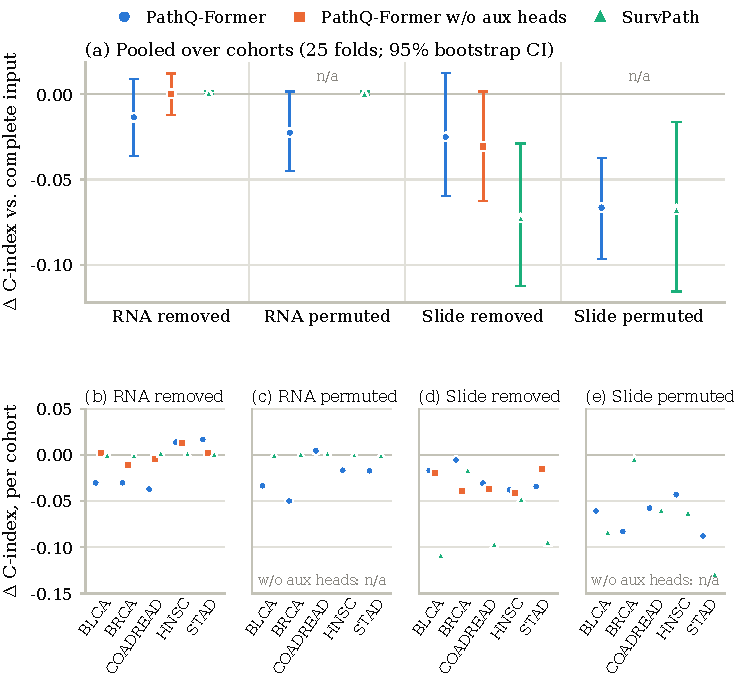
\includegraphics[width=0.69\textwidth]{figures/audit_deltas}
\caption{Change in \cindex{} of the same 20-epoch checkpoint when one test-time input is removed or permuted across validation patients, relative to its complete-input evaluation. In the legend, `w/o aux heads' is the variant without auxiliary heads. SurvPath receives the training-mean gene vector or patch embedding for a removed input; \pq{} uses its learned null codes. (a) Pooled over the five cohorts: per (cohort, fold) the change is averaged over three seeds, then the mean and 95\% bootstrap confidence interval over the 25 folds are shown (10,000 resamples of folds). (b)--(e) The same quantity per cohort (mean over five folds). The variant without auxiliary heads was not evaluated under permutation (n/a).}
\label{fig:audit}
\end{figure*}

The risk-score correlations say how the fused prediction is composed. For \pq{}, the Spearman $\rho$ between the fused risk and the same checkpoint's RNA-removed risk is 0.83 pooled over folds and seeds, against 0.45 with its slide-removed risk, and the two single-input risks correlate at 0.15 (Supplementary Table~S9). The fused prediction therefore remains histology-led: the auxiliary heads make it respond to RNA, they do not make the two inputs symmetric. Its correlations with the other models' risks are in Supplementary Table~S9.

\subsection{Accuracy at Equal Budget}
\label{sec:accuracy}
Table~\ref{tab:acc} gives the \cindex{} of every method and Table~\ref{tab:tests} the seed-averaged paired tests (Supplementary Table~S4 adds the unimodal baselines). Pooled over 25 folds, \pq{} exceeds SurvPath by 0.036 (95\% CI $[-0.004, +0.071]$; $t$-test $p = 0.074$, Wilcoxon $p = 0.030$; 18 of 25 folds) and the variant without auxiliary heads by 0.037 ($[+0.009, +0.065]$; $p = 0.020$ and $0.020$; 17 of 25). Per cohort, BRCA is the only cohort with a raw $p < 0.05$ ($+0.086$, $t$-test $p = 0.017$), and it does not survive Holm correction over the five cohorts ($p = 0.084$); no DSS cohort survives correction (Supplementary Table~S5). Against the RNA-only MLP the margins are $+0.012$ and $+0.014$ ($p \ge 0.34$), and against the late-fusion ensemble $+0.011$ and $+0.009$ ($p \ge 0.28$; seeds 0--1); the MLP scores higher than \pq{} on BRCA and COADREAD and higher than the variant without auxiliary heads on BLCA and BRCA. No unimodal baseline differs from SurvPath pooled (ABMIL $+0.001$, SNN $-0.007$, MLP $+0.024$). The equal-budget result is therefore parity with the best unimodal baseline, not superiority. On overall survival (one seed) \pq{} leads SurvPath by 0.034 ($[+0.014, +0.054]$; $p = 0.003$ and $0.003$), and under a 10-epoch budget the variant without auxiliary heads leads by 0.028 ($p = 0.079$ and $0.063$); both are tabulated in Supplementary Tables~S6 and~S7. Uno's IPCW \cindex{} tracks Harrell's (Supplementary Table~S8): pooled over the 25 seed-averaged folds, it exceeds SurvPath's by 0.039 for \pq{} and 0.046 for the variant without auxiliary heads (Wilcoxon $p = 0.042$ for both; $t$-test $p = 0.153$ and $0.045$), and the integrated Brier score is lower than SurvPath's by 0.070 and 0.071 ($p < 0.001$; $n = 24$, one BRCA fold being undefined), as it is for ABMIL ($-0.068$) and the RNA MLP ($-0.075$). SurvPath's Brier score is the highest on every cohort (0.11--0.34): its published loss weights the censored term by 0.5 and leaves its hazards poorly calibrated under this protocol, so the Brier comparison is reported for completeness only.

\begin{table*}[!t]
\caption{Disease-specific survival \cindex{} under the 20-epoch protocol: mean $\pm$ sample standard deviation over seeds of the five-fold mean (three seeds; late fusion two seeds; the BRCA cells of the single-modality \pq{}s two seeds). Pooled is the mean of the five cohort means. $^\dagger$Development cohort.}
\label{tab:acc}
\centering
\footnotesize
\begin{tabular}{@{}llcccccc@{}}
\toprule
Method & Inputs & BLCA$^\dagger$ & BRCA & COADREAD & HNSC & STAD & Pooled \\
\midrule
\pq{} & WSI+RNA & \pmv{0.630}{0.010} & \pmv{0.622}{0.033} & \pmv{0.613}{0.023} & \pmv{0.582}{0.025} & \pmv{0.572}{0.022} & 0.604 \\
\pq{} without aux.\ heads & WSI+RNA & \pmv{0.609}{0.016} & \pmv{0.611}{0.039} & \pmv{0.638}{0.031} & \pmv{0.575}{0.012} & \pmv{0.593}{0.015} & 0.605 \\
SurvPath & WSI+RNA & \pmv{0.594}{0.012} & \pmv{0.536}{0.026} & \pmv{0.570}{0.038} & \pmv{0.552}{0.019} & \pmv{0.587}{0.008} & 0.568 \\
Late fusion & WSI+RNA & \pmv{0.629}{0.018} & \pmv{0.606}{0.020} & \pmv{0.620}{0.069} & \pmv{0.571}{0.009} & \pmv{0.544}{0.006} & 0.594 \\
ABMIL & WSI & \pmv{0.566}{0.011} & \pmv{0.575}{0.004} & \pmv{0.587}{0.023} & \pmv{0.562}{0.028} & \pmv{0.553}{0.020} & 0.569 \\
Slide-only \pq{} & WSI & \pmv{0.592}{0.003} & \pmv{0.615}{0.027} & \pmv{0.574}{0.024} & \pmv{0.585}{0.003} & \pmv{0.582}{0.019} & 0.590 \\
SNN & RNA & \pmv{0.590}{0.009} & \pmv{0.558}{0.013} & \pmv{0.572}{0.028} & \pmv{0.535}{0.006} & \pmv{0.549}{0.009} & 0.561 \\
RNA MLP & RNA & \pmv{0.611}{0.012} & \pmv{0.627}{0.013} & \pmv{0.633}{0.016} & \pmv{0.555}{0.012} & \pmv{0.532}{0.009} & 0.592 \\
RNA-only \pq{} & RNA & \pmv{0.608}{0.020} & \pmv{0.559}{0.001} & \pmv{0.598}{0.035} & \pmv{0.554}{0.013} & \pmv{0.511}{0.005} & 0.566 \\
\bottomrule
\end{tabular}
\end{table*}

\begin{table*}[!t]
\caption{Seed-averaged paired tests over the 25 pooled (cohort, fold) units: mean difference in \cindex{} (first minus second method), 95\% percentile-bootstrap CI (10,000 resamples of folds), paired $t$-test and exact Wilcoxon $p$-values, and folds won. Seeds are averaged per fold before pairing (three seeds for DSS; seeds 0--1 against late fusion; one seed for OS). The unimodal baselines against SurvPath are in Supplementary Table~S4.}
\label{tab:tests}
\centering
\footnotesize
\begin{tabular}{@{}llrlccc@{}}
\toprule
Comparison & Setting & $\Delta$ & 95\% CI & $t$ $p$ & W $p$ & Wins \\
\midrule
\pq{} vs SurvPath & DSS & $+0.036$ & $[-0.004, +0.071]$ & 0.074 & 0.030 & 18/25 \\
\pq{} without aux.\ heads vs SurvPath & DSS & $+0.037$ & $[+0.009, +0.065]$ & 0.020 & 0.020 & 17/25 \\
\pq{} vs RNA MLP & DSS & $+0.012$ & $[-0.022, +0.044]$ & 0.47 & 0.34 & 14/25 \\
\pq{} without aux.\ heads vs RNA MLP & DSS & $+0.014$ & $[-0.023, +0.049]$ & 0.47 & 0.37 & 16/25 \\
\pq{} vs late fusion & DSS, seeds 0--1 & $+0.011$ & $[-0.013, +0.034]$ & 0.39 & 0.28 & 14/25 \\
\pq{} without aux.\ heads vs late fusion & DSS, seeds 0--1 & $+0.009$ & $[-0.020, +0.036]$ & 0.54 & 0.52 & 14/25 \\
\pq{} vs SurvPath & OS, seed 0 & $+0.034$ & $[+0.014, +0.054]$ & 0.003 & 0.003 & 19/25 \\
\pq{} without aux.\ heads vs SurvPath & DSS, 10 epochs & $+0.028$ & $[-0.001, +0.057]$ & 0.079 & 0.063 & 18/25 \\
\bottomrule
\end{tabular}
\end{table*}

\subsection{Missing Inputs at Test Time}
\label{sec:missing}
Fig.~\ref{fig:missing} shows the random-missingness sweep. With half of the validation patients missing one modality, the fused \cindex{} of \pq{} changes by at most 0.025 (BRCA, 0.622 to 0.597) and that of the variant without auxiliary heads by at most 0.018 (BRCA). For \pq{} every change is within one sample seed standard deviation of the complete-input score (Table~\ref{tab:acc}); for the variant without auxiliary heads the HNSC and STAD changes (0.013 and 0.017) exceed it by 0.001 and 0.002. A site with mixed availability can instead route slide-only patients to ABMIL and RNA-only patients to the RNA MLP, or average the slide-only and RNA-only models when both inputs exist; routing and late fusion are robust by construction, and the late-fusion ensemble matches the joint model (Table~\ref{tab:tests}). What the single checkpoint offers over routing is operational: one model to validate, version and monitor, and one output head whose risks are produced the same way for every patient; whether those risks are comparable across missingness patterns was not tested. The one-checkpoint result is about coverage, not accuracy: with the RNA removed, the single \pq{} checkpoint scores 0.576--0.600 against 0.553--0.587 for ABMIL (higher on four cohorts, lower on COADREAD); with the slide removed it scores 0.538--0.617 against 0.532--0.633 for the RNA MLP, higher on BLCA and STAD and lower on BRCA, COADREAD and HNSC (by up to 0.050 on COADREAD; three-seed means throughout).

\begin{figure*}[!t]
\centering
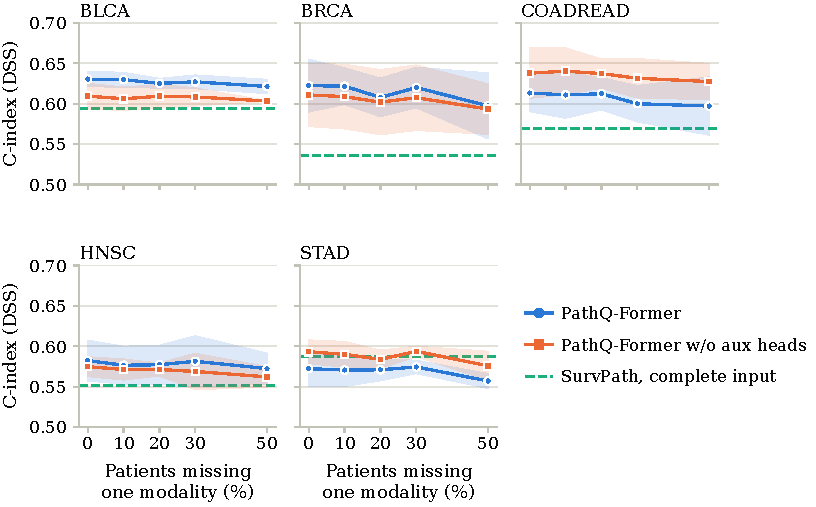
\includegraphics[width=0.76\textwidth]{figures/missing_rate_seeds}
\caption{\cindex{} of \pq{} and of its variant without auxiliary heads (`w/o aux heads' in the legend; 20 epochs) when 0--50\% of validation patients are missing one modality at random (mean of five random draws per fold). Lines: mean over three seeds of the five-fold mean; bands: $\pm$1 sd over seeds. Dashed line: SurvPath with complete inputs (three-seed mean). With half the patients missing a modality the fused \cindex{} changes by at most 0.025 (BRCA).}
\label{fig:missing}
\end{figure*}

\subsection{Where the Robustness Comes From}
\label{sec:where}
Evaluating the same checkpoints under mean imputation instead of the null code separates the two. For the variant without auxiliary heads, replacing the removed slide by the training-mean patch embedding instead of the null code turns a loss of 0.030 into a loss of 0.069 ($t$-test $p = 3 \times 10^{-4}$, Wilcoxon $p = 2.5 \times 10^{-4}$; one seed, 25 folds), the size of SurvPath's collapse; with the heads the loss is 0.035 under mean imputation ($p = 0.040$ and $0.045$; three seeds) against 0.025 with the null code (per-cohort values in Supplementary Table~S10). The attribution is therefore: null codes and modality dropout remove the collapse without the slide; the auxiliary heads make the fused output respond to RNA; and the fused risk remains histology-led ($\rho$ 0.83 against 0.45). Fusion-block ablations on BLCA under the 10-epoch budget (one seed) move the fused \cindex{} within 0.595--0.638, inside the fold standard deviation of 0.07--0.13 (Supplementary Table~S12). Under the 20-epoch budget on BLCA (one seed, trained on a CPU), capping \pq{} at the 4,096 training patches per slide that SurvPath uses gives 0.626 against 0.625 for the seed-0 run with all patches (0.630 $\pm$ 0.010 over three seeds), so on this cohort the margin over SurvPath is not explained by \pq{} reading more patches; two or eight time bins give 0.628 and 0.609, the 281 Xena pathway groups~\cite{goldman2020xena} 0.628 and the 50 Hallmark gene sets alone 0.600, all within one fold standard deviation (Supplementary Table~S13).

\subsection{Checkpoint Selection on Event-Poor Folds}
\label{sec:selection}
Every run stores its per-epoch validation history, so the effect of a selection rule can be replayed without training. Supplementary Table~S11 replays validation-loss early stopping with patience 5 on the 590 stored fold histories of the eight 20-epoch methods. The rule selects epoch 1 on median (mean 1.6; 93\% of folds epoch 1--3) and would have stopped after 6.6 of 20 epochs on average, with the patience limit reached in every fold. Pooled over the 25 seed-averaged folds, the early-stopped checkpoint scores below the final one by 0.090 for \pq{} without heads, 0.059 for \pq{}, 0.065 for the slide-only and 0.034 for the RNA-only \pq{}, 0.038 for SNN and 0.027 for the RNA MLP, and by nothing for ABMIL ($-0.001$) and SurvPath ($+0.000$). The histories show why: ABMIL and SurvPath reach their best validation \cindex{} at epoch 6.2 and 6.9 on average, SNN and the MLP at 7.2--7.3, and the \pq{} variants, which train with a warm-up epoch and a lower learning rate (Supplementary Table~S3), at 9.3--10.0, so an epoch-1--2 checkpoint costs them most. Conversely, under the oracle rule (the epoch of highest validation \cindex{}, an unattainable bound biased in favour of every method) the pooled \cindex{} is 0.67--0.68 for SurvPath, ABMIL, SNN and the RNA MLP and 0.69 for both \pq{} variants (Supplementary Table~S11), so the margin in Table~\ref{tab:tests} depends on the fixed-budget, final-checkpoint rule as well as on the models. Under the replayed rule 23 of the 40 method $\times$ cohort cells have a mean \cindex{} within 0.45--0.55, against 5 under the final checkpoint (HNSC 8 of 8, STAD 7 of 8, BRCA 4 of 8). An earlier validation-loss campaign on these cohorts (patience 5, minimum 6 epochs; 145 folds) behaved the same way: median selected epoch 1 (82\% of folds epoch 1--3) and 14 of 25 method $\times$ cohort cells within 0.45--0.55 (Supplementary Section~S-VIII). Every replayed rule selects and scores on the same fold, so the measured deficit of early stopping is conservative. On cohorts with 5--45 events per validation fold, checkpoints should not be selected on the validation negative log-likelihood; a fixed budget with the final checkpoint, or at least the selected epochs and the events per fold, should be reported.

\section{Discussion}
\label{sec:discussion}

\textit{A general lesson.} Fusion of a strong and a weak modality can converge to ignoring the weak one with no accuracy signal: the fused \cindex{} of the SurvPath checkpoints trained here is as high as their slide-only behaviour permits, and nothing in the survival objective penalises leaving the genomic branch unused once the fusion block has found a low-loss route through the histology branch. This is the modality-competition effect that Gradient Blending~\cite{wang2020gradientblending} and OGM-GE~\cite{peng2022ogmge} describe for classification, and the same remedies apply: per-modality supervision supplies a direct gradient to the weak branch. The audit detects the failure without any training: removal and permutation across patients, with the risk-score correlation, show which input a ranking responds to, and they should accompany any multimodal \cindex{}. Unimodal supervision makes the fused output respond to RNA, but the fused risk still correlates at 0.83 with the same checkpoint's RNA-removed risk and at 0.45 with its slide-removed risk, and the RNA-permuted loss (0.023) is a third of the slide-permuted loss (0.067).

\textit{The RNA-only baseline.} A two-layer MLP on bulk expression, run with repository defaults, matches both fusion variants pooled and scores higher than \pq{} on two of five cohorts. This baseline is cheap and seldom reported at equal budget; without it, an improvement attributed to fusion may be an improvement attributable to the genomic branch. Separating ``pathway tokens help'' from ``fusion helps'' would need an MLP that receives the same pathway tokens, which we have not run.

\Needspace{4\baselineskip}
\textit{Limitations.}
\begin{itemize}
\item \textbf{Baseline tuning and variant selection.} SurvPath was not re-tuned, and \pq{}'s hyper-parameters and the auxiliary-head variant were chosen as described under Scope of claims and in Supplementary Section~S-II. The accuracy comparison is favourable to \pq{} by an amount that cannot be bounded without tuning the baseline, and its margin shrinks to about 0.01 under oracle selection (Section~\ref{sec:selection}).
\item \textbf{Recipe on other architectures.} Null codes, modality dropout and auxiliary heads have not been applied to SurvPath, so how much of the robustness is specific to the query bottleneck is untested.
\item \textbf{Seeds and statistics.} Three seeds for the main comparison, two for late fusion, one for OS. Per-cohort tests have five folds; the fold-level standard deviation of the \cindex{} is 0.12--0.25 on COADREAD for the fusion models (0.05--0.25 over all methods), fold 3 of BLCA is weak for every method except the RNA-only \pq{}, and fold 0 of COADREAD, with five events, scores 0.85--0.92 for \pq{} across seeds. No per-cohort DSS difference survives correction; on OS (one seed) BLCA, the development cohort, does under the $t$-test only (Holm $p = 0.039$; Wilcoxon 0.312). The RNA-permuted loss of 0.023 that supports the auxiliary-head claim has $p = 0.075$ and $0.063$ over 25 folds.
\item \textbf{Data and clinical use.} TCGA only, with frozen UNI2-h features whose pretraining corpus may include TCGA slides, which would make every WSI-based result optimistic; no external cohort; missingness simulated at random, so informative missingness is not covered; no clinical covariates (stage, grade, age), so whether any model adds to them is untested; performance across sex, race and age subgroups was not evaluated. The model is a research prototype evaluated on public, de-identified data, intended for research-grade risk stratification of a cohort with mixed data availability from one model, not for patient-level decision support, and it must not be used to inform patient care.
\end{itemize}

\section{Conclusion}
\label{sec:conclusion}
A fused histology--transcriptomics survival model can score well while its ranking ignores one input: the official SurvPath implementation, under an equal-budget protocol on five TCGA cohorts, does not respond to its RNA input and collapses without the slide. Removal and permutation audits with risk-score correlations detect this and should be reported with any multimodal \cindex{}. Training one fusion model with null codes and modality dropout removes the collapse, and auxiliary unimodal heads make the fused prediction respond to RNA; the resulting single checkpoint serves complete, slide-only and RNA-only patients; with both inputs it is not detectably different from an RNA-only MLP or a late-fusion ensemble, and with one input absent it stays within 0.05 of the dedicated unimodal baseline. Replaying checkpoint selection on the stored histories shows that validation-loss early stopping would have selected epoch 1--3 checkpoints and penalised the late-learning models on these event-poor folds, which argues for fixed budgets and for reporting selected epochs and events per fold.

\section*{Data and Code Availability}
TCGA data are public and de-identified. UNI2-h patch features~\cite{uni2h,uni2hfeatures} and the RNA-seq matrices, clinical metadata and splits released with SurvPath~\cite{jaume2024survpath} are available from their authors. The code (MIT licence), configuration files, archived per-run results (results, configuration, per-fold predictions and training histories for every run; inventory in Supplementary Section~S-VIII) and the script that regenerates every table in Section~\ref{sec:results} and Supplementary Section~S-III are public at \url{https://github.com/SharoonSharif/PathQFormer} and archived at Zenodo (\url{https://doi.org/10.5281/zenodo.22900123}). The 275 trained fold models (\pq{} and its variant without auxiliary heads at three seeds, SurvPath and the slide-only and RNA-only \pq{}s at seed 0, on the five cohorts, plus the two OS runs: 11 run configurations $\times$ five cohorts $\times$ five folds; 18 GB) are on the Hugging Face Hub at \url{https://huggingface.co/sharoonsharif1/PathQFormer-checkpoints}. The supplementary material (one PDF) contains the protocol and methods tables, the model equations and training configuration, the full tables, compute cost, pathway attention, Kaplan--Meier curves, evaluation pitfalls and the run inventory.

\section*{Acknowledgment}
The results published here are in whole or part based upon data generated by the TCGA Research Network (\url{https://www.cancer.gov/tcga}). The author thanks the SurvPath authors and the Mahmood Lab for releasing their code, data splits, pathway definitions and the UNI2-h patch features. A large language model (Claude, Anthropic) assisted with drafting and editing the text and \LaTeX{} source and with writing analysis and plotting code, under the author's direction; the author designed the study, ran the experiments, checked every reported number against the archived results, and is responsible for all content. This work received no dedicated funding; cloud compute was paid for by the author. The author declares no competing interests.

\bibliographystyle{IEEEtran}
\bibliography{references}

\end{document}
